\addtocontents{toc}{\setcounter{tocdepth}{3}}

\chapter{Contexte général}
\section*{Introduction}
Ce chapitre constitue le point de départ du rapport de stage de fin d'études. Nous allons commencer tout d’abord par présenter l'organisme d'accueil SOFRECOM et sa filiale SOFRECOM Tunisie. Nous allons énoncer par la suite la problématique et les objectifs de notre projet et enfin nous allons spécifier la méthodologie et la planification de travail pour sa réalisation.


% Une section

% Exemple d'une section qui porte une référence à une bibliographie
% NB: il faut bien suivre le syntaxe pour ne pas tomber dans le cas où il y a une référence dans la table des matières.
\section[Présentation de l'organisme d'accueil : SOFRECOM]{Présentation de l'organisme d'accueil : SOFRECOM }
Nous allons présenter dans cette section notre organisme d'accueil.
    \subsection{Groupe Sofrecom}
    Sofrecom, filiale d’Orange, développe depuis 50 ans un savoir-faire unique dans les métiers de l’opérateur, ce qui en fait un leader mondial du conseil et de l’ingénierie télécom. Ces dernières années, plus de 200 acteurs majeurs, dans plus de 100 pays, ont confié à Sofrecom la conduite de leurs projets stratégiques et opérationnels. Le réseau de savoir-faire de Sofrecom (Know-How Network) garantit également le transfert de connaissances et de compétences pour une évolution continue basée sur des méthodologies certifiées internationalement \cite{Sofrecom}.
     \subsection{Sofrecom Tunisie }
     Sofrecom Tunisie lancée en Octobre 2012, est la plus jeune et la plus importante filiale du groupe Sofrecom en zone Afrique et Moyen Orient. En 5 ans, elle a pu se positionner en tant qu’un leader d’ingénierie en télécommunications. Sofrecom Tunisie compte aujourd’hui 500 experts, et deux clients majeurs qui font partie du groupe Orange:  Orange Labs Services ( OLS ) et Direction des Systèmes d'Inforamtion ( DSI ) France. Sofrecom Tunisie propose à ses clients une gamme riche de prestations organisées autour de huit métiers \cite{SofrecomTunisie} :
     
     \begin{itemize}
    \item Ingénierie;
    \item Architecture;
    \item Support et maintenance;
    \item Sécurité informatique.
    \item Expertise technique.
    \item Développement;
    \item Innovation;
    \item Consulting.
    \end{itemize}
    Notre projet concerne le métier du développement.
% On peut ajouter une figure en utilisant le syntaxe suivant:


\section{\'Etude et analyse de l'existant }
Dans cette section, nous allons effectuer l'analyse et le critique de l'existant.
    \subsection{Analyse de l’existant}
La direction resources humaine de Sofrecom utilise une application web développée en 2017 pour l'aider à prendre de la décision concernant la démission de ses employés dans le futur.
Cette application est basée sur un système d'information open source H2o.ai permettant la création des modèles d'apprentissage automatique.

Pour construire un modèle de prédiction de "Turnover" de Sofrecom, l'utilisateur de ressource humaine collecte d'abord des données dans un fichier d'extension ".csv" qui représente les caractérestiques des employés (nom, age, matricule, expérience, école, manager, département...).
Après cette phase, l'utilisateur importe ce fichier dans le système d'information H2o.ai.\\ 
Enfin, il effectue plusieurs tâches sur ce fichier telles que:  analyse de fichier, choix des arguments de modèle à construire, choix de variable à prédire (qui est la démission dans notre cas) et sélection d'algorithme pour la construction de modèle afin d'effectuer des prédictions. 

 \subsection{Critique de l’existant}
L'application développée contient plusieurs contraintes :
\begin{itemize}
    \item Téléchargement et activation d'un module dans le navigateur permettant à l'application d'accéder à les services offertes par le système H2o.ai;
     \item Lenteur dans la gestion des prédictions de la démission des employés;
     \item Utilisation d'une solution générique de prédiction;
      \item Lors de la fermeture de système d'information H2o.ai, il n'y aura pas de trace sur les modèles crées ainsi que l'historique de prédiction;
        \item Modèle de prédiction n'est pas performant.
\end{itemize}
\newpage
Cette manière de procéder a un impact négatif sur le traitement de l’information des employés pouvant engendrer des pertes de temps considérables et de grands risques de perte des résultats de prédiction d’où la nécessité d’une application qui a pour but d’optimiser la gestion, le traitement et l’organisation de ces informations.
\section{Problématique}
Sofrecom utilise une application basée sur la plateforme de l'apprentissage automatique H2o.ai.
Elle utilise cette application pour traiter leurs propres informations afin de faire des prédictions pour la démission de ses employés à l'avenir.\\
Le modèle de prédiction développé par H2o.ai ne permet pas de répondre aux nouvelles données mise à jour de Sofrecom et même pour accéder aux services de H2o.ai, il faudra installer un module dans le navigateur pour chaque utilisateur.\\
Face aux difficultés rencontrées, une décision a été prise pour le développement d’une solution propre et spécifique à la société Sofrecom permettant de remédier à ces problèmes afin d'optimiser ces différentes tâches pour faciliter le traitement de prédiction et construire un modèle de prédiction de turnover performant.




\section{Solution proposée}
La solution proposée consiste à développer et implémenter une application propre et spécifique à la société Sofrecom basée sur un modèle d'apprentissage automatique de TURNOVER performant.
L'application propose une visualisation des différentes informations des employés de Sofrecom et permet d'effectuer des prédictions en une seule action sans avoir recours aux différentes autres activités (import de fichier, analyse, choix de variable à prédire...), elle permet de garder l'historique de cette dernière et d'exposer un tableau de bord dynamique.


\section{Méthodologie de développement à adopter : SCRUM}

   
Dans tous les secteurs d’activités, la seule manière possible pour arriver à atteindre les objectifs du travail à réaliser est de suivre une démarche bien précise sur laquelle vont reposer toutes les étapes du projet en cours.\\
Afin d'atteindre nos objectifs et de développer notre application informatique le plus rapidement possible, notre choix a été fixé sur la méthodologie SCRUM. En effet, il s’agit de la meilleure méthodologie itérative qui peut être adaptée dans le cadre de notre projet vue qu'elle a été conçue pour améliorer la productivité dans les équipes auparavant paralysées par des méthodologies classiques.

\subsection{Rôles dans SCRUM}
Le "Product owner" est la personne qui porte la vision du produit à réaliser, responsable de la gestion du "product backlog" et travaille en interaction avec l’équipe de développement. Il s’agit généralement d’un expert du domaine métier du projet. M. Khaled Ksontini est le "Product owner". Le "Scrum master" est la personne qui doit maitriser SCRUM et s’assurer que ce dernier est bien compris et appliqué. M.Aymen BEL ARBI est le "Scrum master". L’équipe transforme les besoins en fonctionnalités pour aboutir à un incrément utilisable et livrable à la fin de chaque itération. L’équipe comporte un étudiant en Génie Logiciel et Systèmes d'Information à l’ISI, qui est le responsable de développement de l'application.\\
Avantages du SCRUM :

 \begin{itemize}
    \item Flexibilité;
    \item Créativité;
    \item Productivité.
    \end{itemize}
    
\subsection{Planification d’un projet par SCRUM}
Pour appliquer correctement SCRUM, il faut comprendre le cycle de vie d’un sprint pendant un processus SCRUM. Le processus, illustré dans la figure \ref{fig:FrameworkScrum }, est décrit ci-dessous :
 \begin{itemize}
    \item le Product owner crée le "product backlog" en déterminant et priorisant les user Story;
    \item Pendant la planification du sprint, l’équipe choisit un ensemble de "user story" les plus prioritaires à partir du "product backlog" pour construire le sprint Backlog;
    \item L’équipe implémente les "user story" pendant une période qui dure de 2 à 4 semaines;
    \item Durant le sprint, l’équipe se réunit chaque jour, "Daily Scrum", pour synchroniser les tâches..
    \item A la fin du sprint, le travail doit être achevé pour faire une démonstration au client;
    \item Le sprint est clôturé par un "sprint review" pour discuter les prochaines étapes du projet et par un "sprint retrospective" pour parler des manières à appliquer pour rendre l’équipe plus productive \cite{scrum}.
    \end{itemize}
    
              \begin{figure}[htpb]
\centering
\fcolorbox{brown}{white}{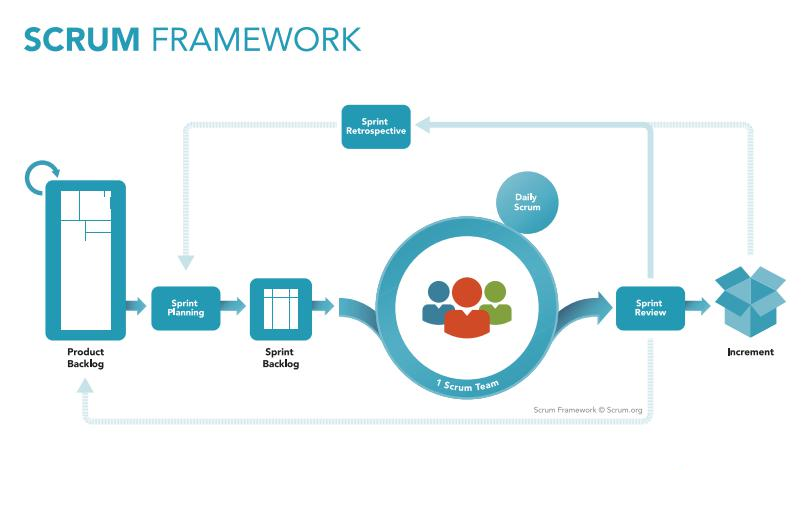
\includegraphics[width=0.8\linewidth]{img/scrum2.png}}
\caption{Le Framework SCRUM}
\label{fig:FrameworkScrum }
\end{figure}
\newpage
   \section{Diagramme de GANTT théorique}
    Le diagramme de la figure ci-après décrit le déroulement chronologique des étapes du stage de fin d'études. Pendant le premier mois, les tâches préliminaires comme la documentation et l’étude théorique du projet ont été effectuées. Ces travaux ont été suivis par l’étude des besoins, qui a abouti à la spécification des besoins et à l’élaboration des diagrammes de cas d’utilisation. Ensuite, la conception et la réalisation de l’application a été mise en oeuvre et ce en parallèle avec son développement pour chaque release. Enfin, le travail réalisé (produit développé) a été testé dans chaque sprint .\\
  
          \begin{figure}[htpb]
 \centering
\fcolorbox{brown}{white}{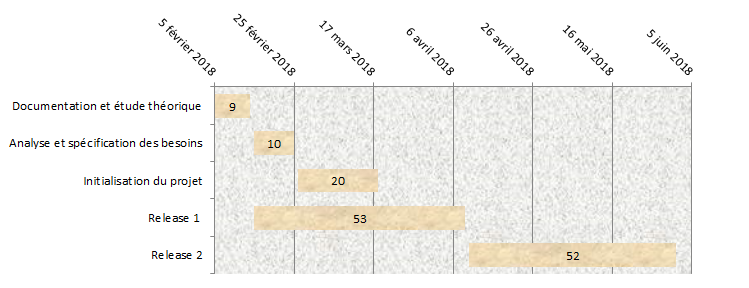
\includegraphics[width=0.8\linewidth]{img/gantt_pfe.png}}
\caption{Diagramme de GANTT théorique}
\label{fig:Diagrammegantt }
\end{figure}

\newpage

\section*{Conclusion}
   Dans ce chapitre, nous avons introduit l’organisme d’accueil Sofrecom. De plus, Nous avons fait l’étude de l’existant et la solution proposée ainsi que la méthodologie adoptée. Le chapitre suivant sera consacré pour l’analyse et la spécification des besoins.
    